\documentclass[border=10pt]{standalone}
\usepackage{tikz}
\usetikzlibrary{shapes, arrows.meta, positioning, calc}

\begin{document}
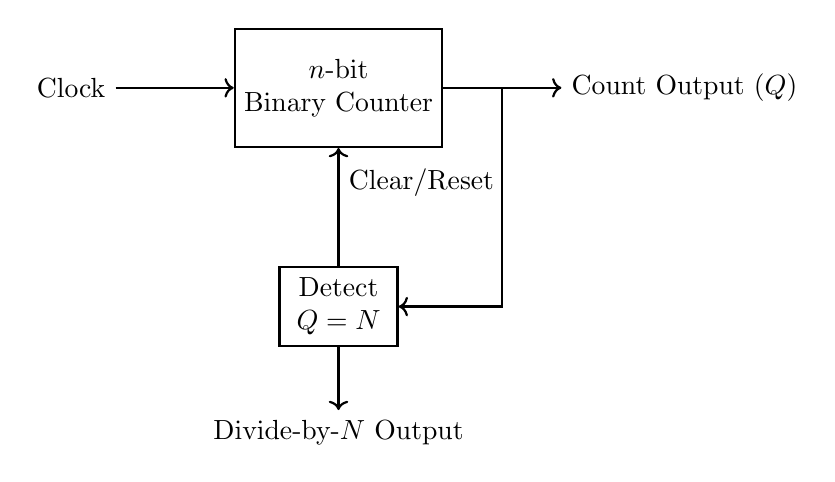
\begin{tikzpicture}[
    auto, 
    node distance=1.5cm, 
    thick,
    block/.style={draw, rectangle, minimum height=1.5cm, minimum width=2.5cm, fill=white, align=center},
    logic/.style={draw, rectangle, minimum height=1cm, minimum width=1.5cm, fill=white, align=center}
]

    % Counter Block
    \node[block] (counter) {$n$-bit\\Binary Counter};
    
    % Inputs
    \node[left=1.5cm of counter.west] (clk) {Clock};
    \draw[->] (clk) -- (counter.west);
    
    % Outputs lines
    \draw[->] (counter.east) -- ++(1.5,0) node[right] (output) {Count Output ($Q$)};
    
    % Tap off outputs for feedback
    \coordinate (tap) at ($(counter.east)!0.5!(output.west)$);
    \node[logic, below=1.5cm of counter] (decoder) {Detect\\$Q=N$};
    
    \draw[->] (tap) |- (decoder.east);
    
    % Feedback to Clear
    % Usually Clear is at bottom or top. Let's assume asynchronous clear at bottom.
    \draw[->] (decoder.north) -- (counter.south) node[midway, above right] {Clear/Reset};
    
    % Label for output of decoder
    \draw[->] (decoder.south) -- ++(0,-0.8) node[below] {Divide-by-$N$ Output};

\end{tikzpicture}
\end{document}
